%\documentclass[12pt,oneside,a4paper]{book}

%\usepackage{amsmath}
%\usepackage{mathtools}
%\usepackage{amsfonts}
%\usepackage{unicode-math}
%\usepackage{geometry}
%\usepackage{ctex}

%\begin{document}

%\setcounter{chapter}{0}
\setcounter{section}{0}
\setcounter{subsection}{0}

\chapter{三维空间}

\begin{dingyi}
在$\R^3$中\\
任取空间中一点$O$,从$O$点做相互垂直的定向直线且按右手螺旋方向依次记为$OX,OY,OZ$\\
则称$[O;X,Y,Z]$为直角坐标系\\
则称$O$为原点,则称$OX,OY,OZ$为坐标轴$(\ $$X$轴, $Y$轴, $Z$轴$)$\\
则称坐标轴决定的平面为坐标平面$(\ $$YZ$平面, $ZX$平面, $XY$平面$)$\\
则称坐标轴定向向外指出的一侧为坐标平面的正面,则称另一侧为坐标平面的反面\\
任取空间中一点$P$,考虑表示正反面的$\pm$和$P$到坐标平面距离,记为有序数组$(x,y,z)$\\
则称$(x,y,z)$为$P$在$[O;X,Y,Z]$上的坐标,则有$|OP|=\sqrt{x^2+y^2+z^2}$
\begin{center}
    \begin{tikzpicture}
    \draw[->] (0,0,0)--(0,0,2) node [below left] {$X$};
    \draw[->] (0,0,0)--(2,0,0) node [right] {$Y$};
    \draw[->] (0,0,0)--(0,2,0) node [above] {$Z$};
    \node at (0,0,0) [left] {$O$};
    \filldraw[black] (1,1,1) circle (2pt) node [above right] {$P$};
    \end{tikzpicture}
\end{center}
\end{dingyi}

\begin{dingyi}
在$\R^3$中\\
取直角坐标系$[O;X,Y,Z]$和空间中一点$P$,有$P$的坐标为$(x,y,z)$\\
则称$\overrightarrow{OP}$与坐标轴定向的夹角为方向角,记为$\alpha,\beta,\gamma\in[0,\pi]$\\
则称$(\cos\alpha,\cos\beta,\cos\gamma)$为$\overrightarrow{OP}$的方向余弦\\
则有$\cos\alpha=\frac{x}{|OP|}, \cos\beta=\frac{y}{|OP|}, \cos\gamma=\frac{z}{|OP|}$\\
则有$\cos^2\alpha+\cos^2\beta+\cos^2\gamma=1$
\begin{center}
    \begin{tikzpicture}
    \draw[->] (0,0,0)--(0,0,2) node [below left] {$X$};
    \draw[->] (0,0,0)--(2,0,0) node [right] {$Y$};
    \draw[->] (0,0,0)--(0,2,0) node [above] {$Z$};
    \node at (0,0,0) [left] {$O$};
    \filldraw[black] (1,1,1) circle (2pt) node [above right] {$P$};
    \draw[dashed] (0,0,0)--(1,1,1);
    \coordinate (X) at (0,0,2);
    \coordinate (Y) at (2,0,0);
    \coordinate (Z) at (0,2,0);
    \coordinate (O) at (0,0,0);
    \coordinate (P) at (1,1,1);
    \pic[draw,angle radius=2mm,"$\alpha$",angle eccentricity=1.6] {angle=X--O--P};
    \pic[draw,angle radius=6mm,"$\beta$",angle eccentricity=1.4] {angle=Y--O--P};
    \pic[draw,angle radius=4mm,"$\gamma$",angle eccentricity=1.4] {angle=P--O--Z};
    \end{tikzpicture}
\end{center}
\end{dingyi}

\begin{dingli}
在$\R^3$中\\
取直角坐标系$[O;X,Y,Z]$和空间中两点$P_1,P_2$\\
若$\overrightarrow{OP_1}$的方向余弦为$(a_1,b_1,c_1)$且$\overrightarrow{OP_2}$的方向余弦为$(a_2,b_2,c_2)$\\
则有$\cos\angle P_1OP_2=a_1a_2+b_1b_2+c_1c_2\ ($余弦定理$)$
\end{dingli}

\begin{dingyi}
在$\R^3$中\\
取直角坐标系$[O;X,Y,Z]$和空间中两点$P_0,P_1$\\
若有$P_0$的坐标为$(x_0,y_0,z_0)$且$\overrightarrow{P_1P_0}=(A,B,C)$\\
则有过$P_0$点且垂直于$P_0P_1$的平面为$A(x-x_0)+B(y-y_0)+C(z-z_0)=0$\\
则称$Ax+By+Cz+D=0$为平面的一般方程\\
若$\sqrt{A^2+B^2+C^2}=1$,则称$Ax+By+Cz+D=0$为平面的法式方程
\end{dingyi}

\begin{dingyi}
在$\R^3$中\\
取直角坐标系$[O;X,Y,Z]$和空间中两点$P_0,P_1$\\
若有$P_0P_1$为平面$A_1x+B_1y+C_1z+D_1=0$和平面$A_2x+B_2y+C_2z+D_2=0$的交线\\
则称$A_1x+B_1y+C_1z+D_1=A_2x+B_2y+C_2z+D_2=0$为直线$P_0P_1$的一般方程\\
若有$P_0$的坐标为$(x_0,y_0,z_0)$且$\overrightarrow{P_1P_0}=(A,B,C)$\\
则称$\frac{x-x_0}{A}=\frac{y-y_0}{B}=\frac{z-z_0}{C}$为直线$P_0P_1$的点向方程\\
则称$x-x_0=tA,y-y_0=tB,z-z_0=tC$为直线$P_0P_1$的参数方程
\end{dingyi}

\begin{dingyi}
在$\R^3$中\\
取直角坐标系$[O;X,Y,Z]$和空间中的两点$P_0,P_1$\\
则称$\overrightarrow{P_0P_1}$为大小为$|P_0P_1|$方向为$P_0\to P_1$的向量\\
一般地,记向量为$\bfa,\bfb,\bfc,\bfx,\bfy\cdots$,大小为$|\bfa|,|\bfb|,|\bfc|,|\bfx|,|\bfy|\cdots$\\
则称$\overrightarrow{P_1P_0}$为$\overrightarrow{P_0P_1}$的相反向量\\
一般地,记向量为$-\bfa,-\bfb,-\bfc,-\bfx,-\bfy\cdots$,有$\overrightarrow{P_1P_0}=-\overrightarrow{P_0P_1}$\\
则称大小为$0$的向量为零向量$\mathbf{0}$,一般地,零向量$\mathbf{0}$的方向为任意方向\\
则称大小为$1$的向量为单位向量
\end{dingyi}

\begin{dingyi}
在$\R^3$中\\
取直角坐标系$[O;X,Y,Z]$和空间中的向量$\bfa=\overrightarrow{P_1P_2},\bfb=\overrightarrow{P_2P_3}$\\
定义向量加法为向量与向量的运算:\\
有三角形法则/平行四边形法则: $\overrightarrow{P_1P_2}+\overrightarrow{P_2P_3}=\overrightarrow{P_1P_3}$
\begin{center}
    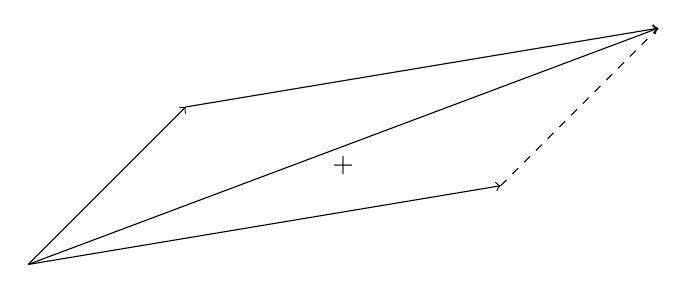
\begin{tikzpicture}
    \coordinate (A) at (0,0);
    \coordinate (B) at (2,2);
    \coordinate (C) at (6,1);
    \coordinate (D) at (8,3);
    \draw[->] (A)--(B) node [left,pos=0.5] {$\bfa$};
    \draw[->] (B)--(D) node [above,pos=0.5] {$\bfb$};
    \draw[->] (A)--(C) node [left,pos=0.5] {$\bfb$};
    \draw[->] (A)--(D) node [below,pos=0.5] {$\bfa+\bfb$};
    \draw[dashed] (C)--(D);
    \end{tikzpicture}
\end{center}
定义向量数乘为实数与向量的运算:\\
有对任意$\lambda\in\R$,则$\lambda\bfa$为大小为$|\lambda||\bfa|$方向为$\sgn(\lambda)\bfa$的向量
\end{dingyi}

\begin{dingli}
在$\R^3$中\\
取直角坐标系$[O;X,Y,Z]$和空间中的向量$\bfa,\bfb,\bfc$\\
则有$\bfa+\bfb=\bfb+\bfa$且$\bfa+(\bfb+\bfc)=(\bfa+\bfb)+\bfc$\\
则有$\bfa+\mathbf{0}=\bfa$且$\bfa+(-\bfa)=\mathbf{0}$\\
则有$|\bfa+\bfb|\leq |\bfa|+|\bfb|$\\
对任意$\lambda,\mu\in\R$\\
则有$\lambda\bfa+\mu\bfa=(\lambda+\mu)\bfa$且$\lambda(\bfa+\bfb)=\lambda\bfa+\mu\bfb$\\
则有$\mu(\lambda\bfa)=(\mu\lambda)\bfa$
\end{dingli}

\begin{dingyi}
在$\R^3$中\\
取直角坐标系$[O;X,Y,Z]$和空间中的向量$\bfa,\bfb$\\
则称向量平移相交后方向夹角为$\bfa,\bfb$的夹角,记为$\langle\bfa,\bfb\rangle\in[0,\pi]$\\
定义向量的内积为向量与向量的运算:\\
有$\bfa\cdot\bfb=|\bfa||\bfb|\cos\langle\bfa,\bfb\rangle$\\
定义向量的外积为向量与向量的运算:\\
有右手螺旋法则:$|\bfa\times\bfb|=|\bfa||\bfb|\sin\langle\bfa,\bfb\rangle,\langle\bfa\times\bfb,\bfa\rangle=\langle\bfa\times\bfb,\bfb\rangle=\frac{\pi}{2}$
\begin{center}
    \begin{tikzpicture}
    \coordinate (O) at (0,0,0);
    \coordinate (A) at (0,0,3);
    \coordinate (B) at (2,0,0);
    \coordinate (C) at (0,2,0);
    \draw[->] (O)--(A) node [left,pos=0.5] {$\bfa$};
    \draw[->] (O)--(B) node [above,pos=0.5] {$\bfb$};
    \draw[->] (O)--(C) node [left,pos=0.5] {$\bfa\times\bfb$};
    \node at (0,0,0) {\Huge\faHandPointRight};
    \end{tikzpicture}
\end{center}
\end{dingyi}

\begin{dingli}
在$\R^3$中\\
取直角坐标系$[O;X,Y,Z]$和空间中的向量$\bfa,\bfb,\bfc$\\
则有$\bfa\cdot\bfb=\bfb\cdot\bfa$且$(\bfa+\bfb)\cdot\bfc=\bfa\cdot\bfc+\bfb\cdot\bfc$\\
则对任意$\lambda\in\R$,有$\lambda(\bfa\cdot\bfb)=(\lambda\bfa)\cdot\bfb$\\
则有$|\bfa\cdot\bfb|\leq|\bfa||\bfb|$\\
则有$\bfa\times\bfb=-\bfb\times\bfa$且$(\bfa+\bfb)\times\bfc=\bfa\times\bfc+\bfb\times\bfc$\\
则对任意$\lambda\in\R$,有$\lambda(\bfa\times\bfb)=(\lambda\bfa)\times\bfb$\\
则有$\bfa\times(\bfb\times\bfc)=(\bfa\cdot\bfc)\bfb-(\bfa\cdot\bfb)\bfc$
\end{dingli}

\begin{dingyi}
在$\R^3$中\\
取直角坐标系$[O;X,Y,Z]$和坐标轴上的单位向量$\bfe_1,\bfe_2,\bfe_3$\\
则有$\bfe_i\cdot\bfe_j=\delta_{ij}$且$\bfe_i\times\bfe_j=\sgn(j-i)\bfe_{6-i-j}$\\
对空间中任意点$P$,有$\overrightarrow{OP}=x\bfe_1+y\bfe_2+z\bfe_3$\\
则称$(x,y,z)$为$\overrightarrow{OP}$的坐标表示,记为$\overrightarrow{OP}=(x,y,z)$
\end{dingyi}

\begin{dingli}
在$\R^3$中\\
取直角坐标系$[O;X,Y,Z]$和向量$\bfa=(x_1,y_1,z_1),\bfb=(x_2,y_2,z_2)$和$\lambda\in\R$\\
则有$\bfa+\bfb=(x_1+x_2,y_1+y_2,z_1+z_2)$且$\lambda\bfa=(\lambda x_1,\lambda x_2,\lambda x_3)$\\
则有$\bfa\cdot\bfb=x_1x_2+y_1y_2+z_1z_2$且$\bfa\times\bfb=(y_1z_2-y_2z_1,z_1x_2-z_2x_1,x_1y_2-x_2y_1)$
\end{dingli}

\chapter{二次曲面}

\begin{dingyi}
在$\R^3$中\\
取直角坐标系$[O;X,Y,Z]$和三元函数$F,F_1,F_2$\\
则称$F(x,y,z)=0$为曲面的一般方程\\
则称$F_1(x,y,z)=F_2(x,y,z)=0$为曲线的一般方程
\end{dingyi}

球面:
\[\frac{x^2}{a^2}+\frac{y^2}{b^2}+\frac{z^2}{c^2}=1\]

\begin{center}
    \begin{minipage}{0.3\textwidth}
        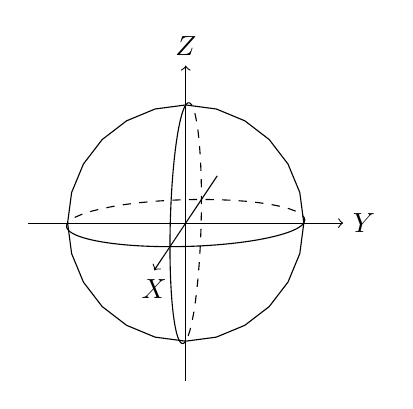
\begin{tikzpicture}[x={(-0.1cm,-0.15cm)},y={(1cm,0cm)},z={(0cm,1cm)}]
        \draw[->] (-4,0,0)--(4,0,0) node[below]{$X$};
        \draw[->] (0,-2,0)--(0,2,0) node[right]{$Y$};
        \draw[->] (0,0,-2)--(0,0,2) node[above]{$Z$};
        \draw plot[domain=0:pi/2] ({2*cos(\x r)},{1.5*sin(\x r)},0);
        \draw[dashed] plot[domain=pi/2:3*pi/2] ({2*cos(\x r)},{1.5*sin(\x r)},0);
        \draw plot[domain=3*pi/2:2*pi] ({2*cos(\x r)},{1.5*sin(\x r)},0);
        \draw plot[domain=0:pi/2] ({2*cos(\x r)},0,{1.5*sin(\x r)});
        \draw[dashed] plot[domain=pi/2:3*pi/2] ({2*cos(\x r)},0,{1.5*sin(\x r)});
        \draw plot[domain=3*pi/2:2*pi] ({2*cos(\x r)},0,{1.5*sin(\x r)});
        \draw plot[domain=0:2*pi] (0,{1.5*cos(\x r)},{1.5*sin(\x r)});
        \end{tikzpicture}
    \end{minipage}
    \hspace{0.5cm}
    \begin{minipage}{0.4\textwidth}
        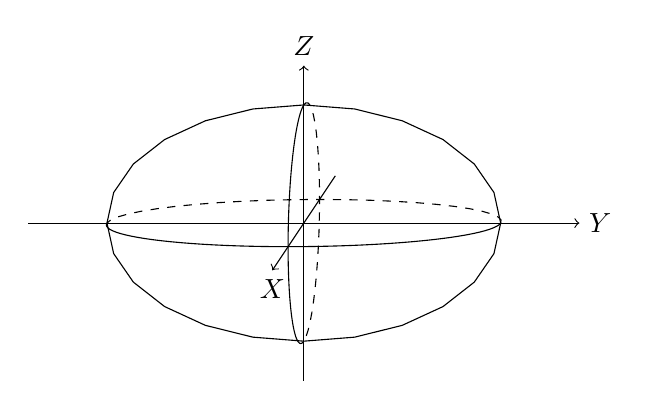
\begin{tikzpicture}[x={(-0.1cm,-0.15cm)},y={(1cm,0cm)},z={(0cm,1cm)}]
        \draw[->] (-4,0,0)--(4,0,0) node[below]{$X$};
        \draw[->] (0,-3.5,0)--(0,3.5,0) node[right]{$Y$};
        \draw[->] (0,0,-2)--(0,0,2) node[above]{$Z$};
        \draw plot[domain=0:pi/2] ({2*cos(\x r)},{2.5*sin(\x r)},0);
        \draw[dashed] plot[domain=pi/2:3*pi/2] ({2*cos(\x r)},{2.5*sin(\x r)},0);
        \draw plot[domain=3*pi/2:2*pi] ({2*cos(\x r)},{2.5*sin(\x r)},0);
        \draw plot[domain=0:pi/2] ({2*cos(\x r)},0,{1.5*sin(\x r)});
        \draw[dashed] plot[domain=pi/2:3*pi/2] ({2*cos(\x r)},0,{1.5*sin(\x r)});
        \draw plot[domain=3*pi/2:2*pi] ({2*cos(\x r)},0,{1.5*sin(\x r)});
        \draw plot[domain=0:2*pi] (0,{2.5*cos(\x r)},{1.5*sin(\x r)});
        \end{tikzpicture}
    \end{minipage}
\end{center}

柱面:
\[F(x,y)=0\]

\begin{center}
    \begin{minipage}{0.2\textwidth}
        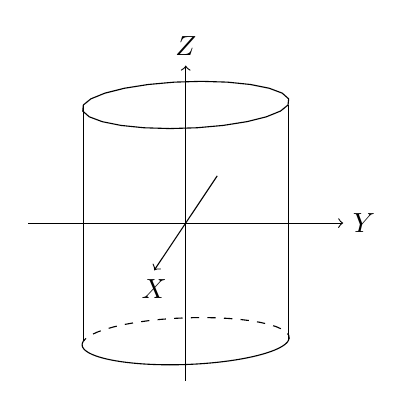
\begin{tikzpicture}[x={(-0.1cm,-0.15cm)},y={(1cm,0cm)},z={(0cm,1cm)}]
        \draw[->] (-4,0,0)--(4,0,0) node[below]{$X$};
        \draw[->] (0,-2,0)--(0,2,0) node[right]{$Y$};
        \draw[->] (0,0,-2)--(0,0,2) node[above]{$Z$};
        \draw plot[domain=0:2*pi] ({2*cos(\x r)},{1.3*sin(\x r)},1.5);
        \draw plot[domain=0:pi/2] ({2*cos(\x r)},{1.3*sin(\x r)},-1.5);
        \draw[dashed] plot[domain=pi/2:3*pi/2] ({2*cos(\x r)},{1.3*sin(\x r)},-1.5);
        \draw plot[domain=3*pi/2:2*pi] ({2*cos(\x r)},{1.3*sin(\x r)},-1.5);
        \draw plot[domain=-1.5:1.5] (0,1.3,{\x});
        \draw plot[domain=-1.5:1.5] (0,-1.3,{\x});
        \end{tikzpicture}
    \end{minipage}
    \hspace{1.5cm}
    \begin{minipage}{0.3\textwidth}
        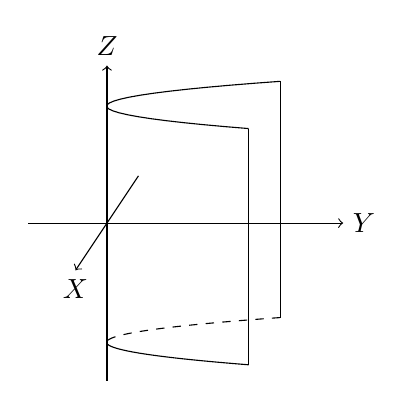
\begin{tikzpicture}[x={(-0.1cm,-0.15cm)},y={(1cm,0cm)},z={(0cm,1cm)}]
        \draw[->] (-4,2,0)--(4,2,0) node[below]{$X$};
        \draw[->] (0,1,0)--(0,5,0) node[right]{$Y$};
        \draw[->] (0,2,-2)--(0,2,2) node[above]{$Z$};
        \draw plot[domain=-2:2] ({\x},{\x*\x/2+2},1.5);
        \draw plot[domain=0:2] ({\x},{\x*\x/2+2},-1.5);
        \draw[dashed] plot[domain=-2:0] ({\x},{\x*\x/2+2},-1.5);
        \draw plot[domain=-1.5:1.5] (0,2,{\x});
        \draw plot[domain=-1.5:1.5] (2,4,{\x});
        \draw plot[domain=-1.5:1.5] (-2,4,{\x});
        \end{tikzpicture}
    \end{minipage}
    \hspace{-0.1cm}
    \begin{minipage}{0.3\textwidth}
        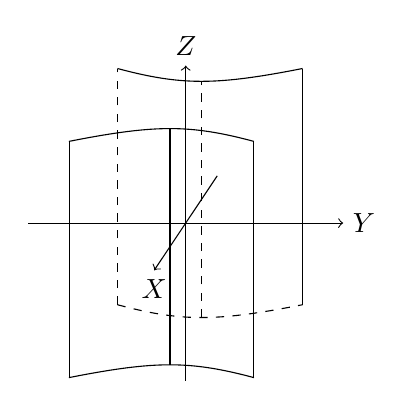
\begin{tikzpicture}[x={(-0.1cm,-0.15cm)},y={(1cm,0cm)},z={(0cm,1cm)}]
        \draw[->] (-4,0,0)--(4,0,0) node[below]{$X$};
        \draw[->] (0,-2,0)--(0,2,0) node[right]{$Y$};
        \draw[->] (0,0,-2)--(0,0,2) node[above]{$Z$};
        \draw plot[domain=-1:1] ({2*cosh(\x)},{sinh(\x)},1.5);
        \draw plot[domain=-1:1] ({-2*cosh(\x)},{sinh(\x)},1.5);
        \draw plot[domain=-1:1] ({2*cosh(\x)},{sinh(\x)},-1.5);
        \draw[dashed] plot[domain=-1:1] ({-2*cosh(\x)},{sinh(\x)},-1.5);
        \draw plot[domain=-1.5:1.5] (3.085,-1.17,{\x});
        \draw plot[domain=-1.5:1.5] (2,0,{\x});
        \draw plot[domain=-1.5:1.5] (3.085,1.17,{\x});
        \draw[dashed] plot[domain=-1.5:1.5] (-3.085,-1.17,{\x});
        \draw[dashed] plot[domain=-1.5:1.5] (-2,0,{\x});
        \draw plot[domain=-1.5:1.5] (-3.085,1.17,{\x});
        \end{tikzpicture}
    \end{minipage}
\end{center}

锥面:
\[F(x,y)=z^2\]

\begin{center}
   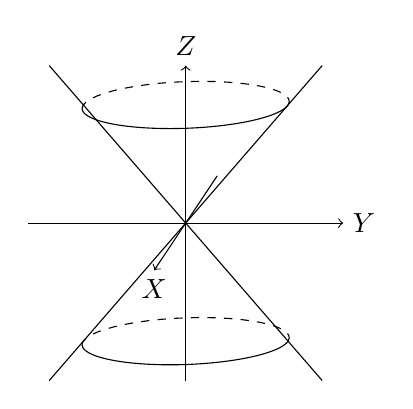
\begin{tikzpicture}[x={(-0.1cm,-0.15cm)},y={(1cm,0cm)},z={(0cm,1cm)}]
    \draw[->] (-4,0,0)--(4,0,0) node[below]{$X$};
    \draw[->] (0,-2,0)--(0,2,0) node[right]{$Y$};
    \draw[->] (0,0,-2)--(0,0,2) node[above]{$Z$};
    \draw plot[domain=0:pi/2] ({2*cos(\x r)},{1.3*sin(\x r)},1.5);
    \draw[dashed] plot[domain=pi/2:3*pi/2] ({2*cos(\x r)},{1.3*sin(\x r)},1.5);
    \draw plot[domain=3*pi/2:2*pi] ({2*cos(\x r)},{1.3*sin(\x r)},1.5);
    \draw plot[domain=0:pi/2] ({2*cos(\x r)},{1.3*sin(\x r)},-1.5);
    \draw[dashed] plot[domain=pi/2:3*pi/2] ({2*cos(\x r)},{1.3*sin(\x r)},-1.5);
    \draw plot[domain=3*pi/2:2*pi] ({2*cos(\x r)},{1.3*sin(\x r)},-1.5);
    \draw plot[domain=-2:2] (0,{1.3*\x/1.5},{\x});
    \draw plot[domain=-2:2] (0,{-1.3*\x/1.5},{\x});
    \end{tikzpicture}
\end{center}

单叶双曲面:
\[\frac{x^2}{a^2}+\frac{y^2}{b^2}-\frac{z^2}{c^2}=1\]

双叶双曲面:
\[\frac{x^2}{a^2}+\frac{y^2}{b^2}-\frac{z^2}{c^2}=-1\]

\begin{center}
    \begin{minipage}{0.4\textwidth}
        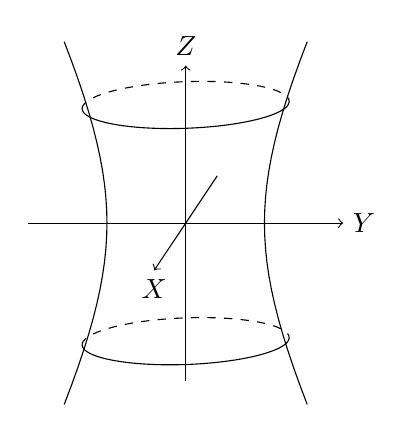
\begin{tikzpicture}[x={(-0.1cm,-0.15cm)},y={(1cm,0cm)},z={(0cm,1cm)}]
        \draw[->] (-4,0,0)--(4,0,0) node[below]{$X$};
        \draw[->] (0,-2,0)--(0,2,0) node[right]{$Y$};
        \draw[->] (0,0,-2)--(0,0,2) node[above]{$Z$};
        \draw plot[domain=0:pi/2] ({2*cos(\x r)},{1.3*sin(\x r)},1.5);
        \draw[dashed] plot[domain=pi/2:3*pi/2] ({2*cos(\x r)},{1.3*sin(\x r)},1.5);
        \draw plot[domain=3*pi/2:2*pi] ({2*cos(\x r)},{1.3*sin(\x r)},1.5);
        \draw plot[domain=0:pi/2] ({2*cos(\x r)},{1.3*sin(\x r)},-1.5);
        \draw[dashed] plot[domain=pi/2:3*pi/2] ({2*cos(\x r)},{1.3*sin(\x r)},-1.5);
        \draw plot[domain=3*pi/2:2*pi] ({2*cos(\x r)},{1.3*sin(\x r)},-1.5);
        \draw plot[domain=-1:1] (0,{cosh(\x)},{1.96*sinh(\x)});
        \draw plot[domain=-1:1] (0,{-cosh(\x)},{1.96*sinh(\x)});
        \end{tikzpicture}
    \end{minipage}
    \hspace{0.5cm}
    \begin{minipage}{0.4\textwidth}
        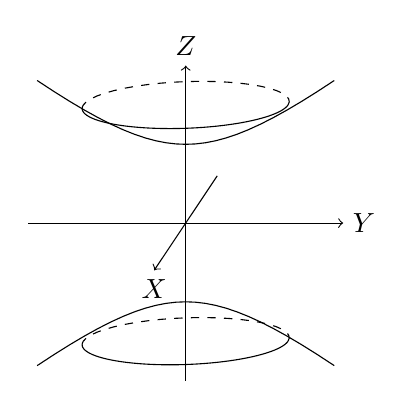
\begin{tikzpicture}[x={(-0.1cm,-0.15cm)},y={(1cm,0cm)},z={(0cm,1cm)}]
        \draw[->] (-4,0,0)--(4,0,0) node[below]{$X$};
        \draw[->] (0,-2,0)--(0,2,0) node[right]{$Y$};
        \draw[->] (0,0,-2)--(0,0,2) node[above]{$Z$};
        \draw plot[domain=0:pi/2] ({2*cos(\x r)},{1.3*sin(\x r)},1.5);
        \draw[dashed] plot[domain=pi/2:3*pi/2] ({2*cos(\x r)},{1.3*sin(\x r)},1.5);
        \draw plot[domain=3*pi/2:2*pi] ({2*cos(\x r)},{1.3*sin(\x r)},1.5);
        \draw plot[domain=0:pi/2] ({2*cos(\x r)},{1.3*sin(\x r)},-1.5);
        \draw[dashed] plot[domain=pi/2:3*pi/2] ({2*cos(\x r)},{1.3*sin(\x r)},-1.5);
        \draw plot[domain=3*pi/2:2*pi] ({2*cos(\x r)},{1.3*sin(\x r)},-1.5);
        \draw plot[domain=-1.2:1.2] (0,{1.25*sinh(\x)},{cosh(\x)});
        \draw plot[domain=-1.2:1.2] (0,{1.25*sinh(\x)},{-cosh(\x)});
        \end{tikzpicture}
    \end{minipage}
\end{center}

椭圆抛物面:
\[\frac{x^2}{a^2}+\frac{y^2}{b^2}=z\]

双曲抛物面:
\[\frac{x^2}{a^2}-\frac{y^2}{b^2}=z\]

\begin{center}
   \begin{minipage}{0.4\textwidth}
        \begin{tikzpicture}[x={(-0.1cm,-0.15cm)},y={(1cm,0cm)},z={(0cm,1cm)}]
        \draw[->] (-4,0,0)--(4,0,0) node[below]{$X$};
        \draw[->] (0,-2,0)--(0,2,0) node[right]{$Y$};
        \draw[->] (0,0,-2)--(0,0,2) node[above]{$Z$};
        \draw plot[domain=0:pi/2] ({2*cos(\x r)},{1.3*sin(\x r)},1.5);
        \draw[dashed] plot[domain=pi/2:3*pi/2] ({2*cos(\x r)},{1.3*sin(\x r)},1.5);
        \draw plot[domain=3*pi/2:2*pi] ({2*cos(\x r)},{1.3*sin(\x r)},1.5);
        \draw plot[domain=-1.5:1.5] (0,{\x},{0.887*\x*\x});
        \end{tikzpicture}
    \end{minipage}
    \hspace{0.5cm}
    \begin{minipage}{0.4\textwidth}
        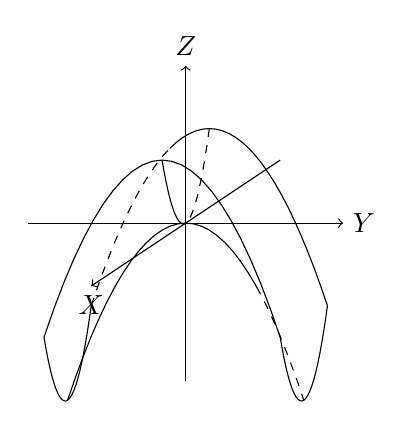
\begin{tikzpicture}[x={(-0.3cm,-0.2cm)},y={(1cm,0cm)},z={(0cm,1cm)}]
        \draw[->] (-4,0,0)--(4,0,0) node[below]{$X$};
        \draw[->] (0,-2,0)--(0,2,0) node[right]{$Y$};
        \draw[->] (0,0,-2)--(0,0,2) node[above]{$Z$};
        \draw[dashed] plot[domain=-1:0] ({\x},0,{\x*\x});
        \draw plot[domain=0:1] ({\x},0,{\x*\x});
        \draw[dashed] plot[domain=-1.5:-0.5] (-1,{\x},{1-\x*\x});
        \draw plot[domain=-0.5:1.5] (-1,{\x},{1-\x*\x});
        \draw plot[domain=-1.5:1.5] (1,{\x},{1-\x*\x});
        \draw plot[domain=-1:1] ({\x},1.5,{\x*\x-2.25});
        \draw plot[domain=-1:1] ({\x},-1.5,{\x*\x-2.25});
        \draw plot[domain=-1.5:0.9] (0,{\x},{-\x*\x});
        \draw[dashed] plot[domain=0.9:1.5] (0,{\x},{-\x*\x});
        \end{tikzpicture}
    \end{minipage}
\end{center}

\chapter{一些变换}

\begin{dingyi}
在$\R^3$中\\
取直角坐标系$[O;X,Y,Z]$和$\overrightarrow{OP}=x\bfe_1+y\bfe_2+z\bfe_3$\\
考虑另一直角坐标系$[O';X',Y',Z']$和$\overrightarrow{O'P}=x'\bfe_1'+y'\bfe_2'+z'\bfe_3'$\\
在$[O;X,Y,Z]$上,记$O',\bfe_i'$的坐标为$(a_1,a_2,a_3),(a_{1i},a_{2i},a_{3i})$\\
则称$\overrightarrow{OP}=\sum\limits_{i=1}^{3}(a_i+\sum\limits_{j=1}^{3}a_{ij})\bfe_i$为$[O;X,Y,Z],[O';X',Y',Z']$的坐标变换公式
\end{dingyi}

\begin{dingyi}
在$\R^3$中\\
若有$\varphi$为空间中点到点的一一对应,则称$\varphi$为变换,则称$\varphi^{-1}$为$\varphi$的逆变换
\end{dingyi}

\begin{dingli}
在$\R^3$中\\
对任意变换$\varphi,\psi,\tau$,则有$\tau\circ(\psi\circ\varphi)=(\tau\circ\psi)\circ\varphi$且$\varphi\circ\id=\varphi$\\
则有存在唯一变换$\varphi^{-1}$,有$\varphi\circ\varphi^{-1}=\varphi^{-1}\circ\varphi=\id$
\end{dingli}

\begin{dingyi}
在$\R^3$中\\
若有变换$\alpha$,对空间中任意点$P$,有$\overrightarrow{P\alpha(P)}$为常向量$\bfa$\\
则称$\alpha$为平移变换\\
则称$\overrightarrow{O\alpha(P)}=\bfa+\overrightarrow{OP}$为平移变换的坐标公式\\
若有变换$\tau$,存在点$P_0$和$\theta\in[0,2\pi)$\\
对任意点$P\in\overline{OP_0}$,有$\tau(P)=P$\\
对任意点$P\notin\overline{OP_0}$,有$\langle\overrightarrow{OP_0}\times\overrightarrow{OP},\overrightarrow{OP_0}\times\overrightarrow{O\tau(P)}\rangle=\theta$\\
则称$\tau$为旋转变换,则称$\overline{OP}$为旋转轴,则称$\theta$为旋转角,记$\bfe=\frac{\overrightarrow{OP_0}}{|OP_0|}$\\
则称$\overrightarrow{O\tau(P)}=(1-\cos\theta)(\bfe\cdot\overrightarrow{OP})\bfe+\cos\theta\overrightarrow{OP}+\sin\theta\bfe\times\overrightarrow{OP}$为旋转变换的坐标公式\\
若有变换$\pi$,存在法向量$\mathbf{n}$确定的过原点平面$\beta$\\
对任意点$P\in\beta$,有$\pi(P)=P$\\
对任意点$P\notin\beta$,有$\overrightarrow{\pi(P)P}\neq\mathbf{0}$且$\overrightarrow{\pi(P)P}\cdot\mathbf{n}=0$且$\overrightarrow{O\pi(P)}\times\mathbf{n}=\overrightarrow{OP}\times\mathbf{n}$\\
则称$\pi$为反射变换,则称$\beta$为反射平面\\
则称$\overrightarrow{O\pi(P)}=\overrightarrow{OP}-2(\overrightarrow{OP}\cdot\mathbf{n})\mathbf{n}$为反射变换的坐标公式\\
若有变换$\varphi$,对空间中任意点$P_1,P_2$,有$|\varphi(P_1)\varphi(P_2)|=|P_1P_2|$\\
则称$\varphi$为正交变换
\end{dingyi}

%\begin{zhu}
%$\overrightarrow{O\tau(P)}=(\bfe\cdot\overrightarrow{OP})\bfe+\cos\theta(\overrightarrow{OP}-(\bfe\cdot\overrightarrow{OP})\bfe)+\sin\theta\bfe\times(\overrightarrow{OP}-(\bfe\cdot\overrightarrow{OP})\bfe)$
%\end{zhu}

\begin{dingli}
在$\R^3$中\\
对任意正交变换$\varphi$,存在平移变换$\alpha$,旋转变换$\tau$,反射变换$\pi$,有$\varphi=\pi\circ\tau\alpha$\\
其中平移变换,旋转变换,反射变换可为$\id$
\end{dingli}

\begin{zhu}
以下用坐标方程组来描述上述变换:\\
对$[O;X,Y,Z],[O';X',Y',Z']$的坐标变换:
\[\begin{cases*}x=a_1+a_{11}x'+a_{12}y'+a_{13}z'\\y=a_2+a_{21}x'+a_{22}y'+a_{23}z'\\z=a_3+a_{31}x'+a_{32}y'+a_{33}z'\end{cases*}\]
有正交条件:
\[\begin{cases*}a_{11}^2+a_{21}^2+a_{31}^2=a_{12}^2+a_{22}^2+a_{32}^2=a_{13}^2+a_{23}^2+a_{33}^2=1\\a_{11}a_{12}+a_{21}a_{22}+a_{31}a_{32}=a_{12}a_{13}+a_{22}a_{23}+a_{32}a_{33}=a_{13}a_{11}+a_{23}a_{21}+a_{33}a_{31}=0\end{cases*}\]
对向量$\bfa=(a_1,a_2,a_3)$的平移变换:
\[\begin{cases*}x'=x+a_1\\y'=y+a_2\\z'=z+a_3\end{cases*}\]
对旋转轴$x=y=0$旋转角$\theta$的平移变换:
\[\begin{cases*}x'=x\cos\theta-y\sin\theta\\y'=x\sin\theta+y\cos\theta\\z'=z\end{cases*}\]
对法向量$(0,0,1)$的反射变换:
\[\begin{cases*}x'=x\\y'=y \\z'=-z\end{cases*}\]
对正交变换:
\[\begin{cases*}x'=a_1+a_{11}x+a_{12}y+a_{13}z\\y'=a_2+a_{21}x+a_{22}y+a_{23}z\\z'=a_3+a_{31}x+a_{32}y+a_{33}z\end{cases*}\]
有正交条件且$\left|\begin{matrix*}a_{11}&a_{12}&a_{13}\\a_{21}&a_{22}&a_{23}\\a_{31}&a_{32}&a_{33}\end{matrix*}\right|=1$
\end{zhu}

%\end{document}